% may be add code snippets here to give a preview of some stuff that had to be done inside Postgres

The main challenge of implementing provenance is maintaining source information at a tuple granulatity, while still remaining consistent with the general structure and invariants of the Postgres executor. In this section, we describe how this data is preserved during the execution of an arbitrary SQL query.

\subsection{Executor}

Since we are concerned with tuple-query level provenance, we only need to preserve information from a single query. We assume that this origin information can always be read directly off of base-level tuples at the beginning of a scan \footnote{This assumption breaks temporary tables, but these can be handled has a special case since there is enough additional information in the \texttt{pg\_prov} table. }. When scanning a base-level tuple, we collect the table id, primary key values, and any other provenance info and pack it into a \texttt{ProvInfo} structure. The goal of this work is to route \texttt{ProvInfo} through the executor from scan to insert.

From a birds-eye view, the executor consists of a collection of node classes, one for each type of plan node. At initialization, it creates a tree of objects representing the query plan given by the optimizer. Each node has its own state and memory context and they communicate with each other through an iterator interface. The payload of this interface is the \texttt{TupleTableSlot} structure, which abstracts over various internal tuple representations. In order to pass information bottom-up to higher nodes, we append the \texttt{ProvInfo}s for the current tuple onto this slot.


\begin{verbatim}
struct TupleTableSlot {
  ...
  List <ProvInfo> provinfos;
}
\end{verbatim}

\begin{figure}
  \scalebox{0.8} {
    
      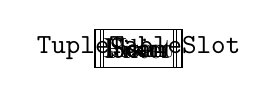
\begin{tikzpicture}
        \Tree [ .\node[draw, rectangle](i1){Insert}; [ .\node[draw, rectangle](j1){Join}; [ .\node[draw, rectangle] (f1) {Filter};  
        \node[draw, rectangle](s1){Scan}; ]  \node[draw, rectangle] (s2) {Scan};  ] ]   

        \path [->] (s2) edge[thick, bend right = 50, dotted] node {\texttt{TupleTableSlot}} (j1);    
        \path [->] (s1) edge[thick, bend left = 50, dotted] (f1);            
        \path [->] (j1) edge[thick, bend right = 50, dotted] (i1);    
        \path [->] (f1) edge[thick, bend left = 50, dotted] (j1);    
        
      \end{tikzpicture}
    }
    \caption {Provenance information is propogated with tuples through the execution plan. }
\end{figure}

Since all nodes communicate through this common interface, provenance information is always preserved through inter node channels. Unfortunately, a node itself may perform arbitary operations on the tuples it receives. We cannot hope to preserve provenence through all nodes, for instance stored procedures, but we can keep this information for standard SQL queries.  
 
\subsubsection{Scans, Filters, and Projections}

The most basic nodes in a query plan are the ones that receive a single input tuple and optionally output a single tuple, e.g. scans, filters, and projections. Postgres implements this style of node as a projection directly on \texttt{TupleTableSlot}. We simply modify this projection function to preserve the \texttt{ProvInfo} from incoming tuple.

\subsubsection{Joins: Hashing and Sorting}

Joins follow a similar interface as scans, they take in a tuple slot and output projected tuples; however internally, they directly access the internal contents of the tuple. Both hash join nodes and sort merge join nodes first convert their input into a set of \texttt{MinimalTuples} before performing the joins. 

The \texttt{MinimalTuple} structure is are direct representation of the tuple data. It is designed to use up minimal memory in cases where many tuples are in kept main memory. When a join is successfully performed, the resulting fields are projected out directly from the \texttt{MinimalTuple} representation. 

In order to preserve provenance, we need to tag every minimal tuple with it provenance information. Fig~\ref{mintup} gives our new minimal tuple representation. In many cases this provenance information will be negligible, but it could be a source of significant slow down. We explore this furthur in Section~\ref{disc}.

This extra tag is the only modification needed to handle joins. When we convert a tuple from a \texttt{TupleTableSlot} to a \texttt{MinimalTuple}, it is tagged with this information. To internal hashing, sorting, and other operations on minimal tuples this information opaque.   

\begin{figure}
  \centering
  \label{mintup}
  \begin{tikzpicture}[node distance=2cm]
    \node [abstract, rectangle split, rectangle split parts=3] {
      Header
      \nodepart{second}Tuple\newline Body
      \nodepart{third}Provenance
    };
  \end{tikzpicture}
  \caption {The modified \texttt{MinimalTuple} tagged with provenance infomation.}
\end{figure}





\subsubsection{Aggregates and Grouping}

The final important special case is for aggregate and grouping nodes. Postgres supports general aggregate operations and so it contains special structures for maintaining aggregate state that break our tuple assumptions. To handle aggregates conservatively, we assume that every tuple that is scanned as part of an  aggregate function should be a part of the provenance information, even if it is ignored in practice. To implement this aggregation strategy, we augment the internal state maintained for each aggregate group to also include the provenance. When the aggregation is advanced by one tuple, we add this tuple's provenance information to the state information. 


\subsection{Insertion of Provenance}

The insertion node has the task of finalizing the provenance. It first inserts the tuple (so that it has a primary key), and then write the tuples \texttt{ProvInfos} to storage. Provenance storage is implemented as a Postgres catalog table called \texttt{pg\_prov} shown in Fig~\ref{pgprov}. The schema represents the information as a directed graph between tuples. Using the catalog for storage is convenient for analysis and visualization, and it opens up the possibility of a special syntax for querying provenance directly. 


\begin{figure}
  \centering
  \label{pgprov}
\texttt{pg\_prov}

\begin{tabular}{|lc|}
  \hline
  Attr & Type \\
  \hline
  origin\_tableid & OID \\
  dest\_tableid & OID \\
  origin\_primary\_key & ARRAY \\
  dest\_primary\_key & ARRAY \\
  command\_id & ID \\
  \hline
\end{tabular}

\texttt{pg\_provcommand}
\begin{tabular}{|lc|}
  \hline
  Attr & Type \\
  \hline
  id & ID \\
  sql & TEXT \\
  \hline  
\end{tabular}
\end{figure}
